\documentclass[a4paper]{article}

%% Language and font encodings
\usepackage[english]{babel}
\usepackage[utf8x]{inputenc}
\usepackage[T1]{fontenc}

%% Sets page size and margins
\usepackage[a4paper,top=2.5cm,bottom=2cm,left=3cm,right=3cm,marginparwidth=1.75cm]{geometry}
\setlength{\parindent}{0pt}

%% Useful packages
\usepackage{amsmath}
\usepackage{amssymb}
\usepackage{physics}
\usepackage{float}
\usepackage{listings}
\usepackage{textpos}
\usepackage{graphicx}
\usepackage[colorinlistoftodos]{todonotes}
\usepackage[colorlinks=true, allcolors=black]{hyperref}
\usepackage[numbered,framed]{matlab-prettifier}

\title{\vspace*{2cm}1.2 Ordinary Differential Equations\vspace*{-1.5cm}}
\date{}

\begin{document}
\maketitle

\begin{textblock*}{100mm}(0cm,-5.5cm)
\Huge 1.2
\end{textblock*}

\section*{Programming Task}
For this programming task I wrote Programming\textunderscore Task.m which includes two functions called FE (Forward Euler) and RK4 (Runge-Kutta 4) which perform the methods specified in the project.

\section*{Question 1}
Adapting my first program to produce Question\textunderscore1.m on running with $h=0.6$ the following output is produced. Note the final column is the estimate of growth rate on the $n^{th}$ iteration calculated by comparing the current and previous $E_n$ values.
\begin{table}[H]
\centering
\begin{verbatim}
       x_n        Y_n            y(x_n)           E_n             gr_n 
       0.0   0.0000000e+00   0.0000000e+00   0.0000000e+00 
       0.6   9.0000000e+00   5.4874391e-01   8.4512561e+00 
       1.2  -7.2460695e+01   3.0119421e-01  -7.2761889e+01   3.5881287e+00 
       1.8   6.2587273e+02   1.6529889e-01   6.2570743e+02   3.5861510e+00 
       2.4  -5.3810178e+03   9.0717953e-02  -5.3811085e+03   3.5862780e+00 
       3.0   4.6277569e+04   4.9787068e-02   4.6277519e+04   3.5862699e+00 
       3.6  -3.9798665e+05   2.7323722e-02  -3.9798667e+05   3.5862704e+00 
       4.2   3.4226854e+06   1.4995577e-02   3.4226854e+06   3.5862703e+00 
       4.8  -2.9435094e+07   8.2297470e-03  -2.9435094e+07   3.5862703e+00 
       5.4   2.5314181e+08   4.5165809e-03   2.5314181e+08   3.5862703e+00 
       6.0  -2.1770196e+09   2.4787522e-03  -2.1770196e+09   3.5862703e+00
\end{verbatim}
\caption{$h=0.6$ gives an estimate for the growth rate of $\gamma \approx 3.5862703$.}
\end{table}

The following tables contain a selection of output from the cases $h=0.4,0.2,0.125,0.1$. \\

Case $h=0.4$
\begin{table}[H]
\centering
\begin{verbatim}
      x_n        Y_n            y(x_n)           E_n            gr_n 
       :          :               :               :               : 
      5.2    3.281395e+09    5.516564e-03    3.281395e+09    4.215997e+00
      5.6   -1.771953e+10    3.697864e-03   -1.771953e+10    4.215997e+00
      6.0    9.568548e+10    2.478752e-03    9.568548e+10    4.215997e+00
\end{verbatim}
\caption{For $h=0.4$ the growth rate is $\gamma \approx 4.22$.}
\end{table}

Case $h=0.2$
\begin{table}[H]
\centering
\begin{verbatim}
      x_n        Y_n            y(x_n)           E_n            gr_n 
       :          :               :               :               : 
      5.6   -3.847086e+09    3.697864e-03   -3.847086e+09    3.942287e+00
      5.8    8.463590e+09    3.027555e-03    8.463590e+09    3.942287e+00
      6.0   -1.861990e+10    2.478752e-03   -1.861990e+10    3.942287e+00
\end{verbatim}
\caption{For $h=0.2$ the growth rate is $\gamma \approx 3.94$.}
\end{table}

Case $h=0.125$
\begin{table}[H]
\centering
\begin{verbatim}
     x_n        Y_n            y(x_n)           E_n            gr_n 
      :          :               :               :               : 
    5.750   -9.928475e-01    3.182781e-03   -9.960303e-01    2.171695e-04
    5.875    9.988152e-01    2.808794e-03    9.960064e-01   -1.916511e-04
    6.000   -9.935487e-01    2.478752e-03   -9.960274e-01    1.691317e-04
\end{verbatim}
\caption{For $h=0.125$ the growth rate is $\gamma \approx 0.00$.}
\end{table}

Case $h=0.1$
\begin{table}[H]
\centering
\begin{verbatim}
      x_n        Y_n            y(x_n)           E_n            gr_n 
       :          :               :               :               : 
      5.8    3.017822e-03    3.027555e-03   -9.732313e-06   -9.999997e-01
      5.9    2.730639e-03    2.739445e-03   -8.806160e-06   -1.000000e+00
      6.0    2.470784e-03    2.478752e-03   -7.968144e-06   -9.999998e-01
\end{verbatim}
\caption{For $h=0.1$ the growth rate is $\gamma \approx -1.00$.}
\end{table}

Reducing $h$ reduces the instability and the growth rate. Reducing $h$ to 0.125 brings the growth rate down to approximately 0 and stabilizes the error. Below 0.125 the instability disappears completely as can be seen in the $h=0.1$ case. 

\section*{Question 2}

\renewcommand{\labelenumi}{\roman{enumi}}
\begin{enumerate}
\item
	The Euler difference equation
	\[ Y_{n+1} = Y_n + h(-16Y_n + 15(e^{-h})^n) \qquad with \qquad Y_0=0 \]
    This can be solved analytically as follows
    \begin{align*}
    Y_n &= (1-16h)Y_{n-1} + 15he^{-nh} \\
    Y_n &= (1-16h)[(1-16h)Y_{n-2} + 15he^{-(n-1)h}] + 15he^{-nh} \\
    \vdots \enspace &= \qquad\qquad\qquad \vdots \\
    Y_n &= (1-16h)^nY_0 + \sum_{i=0}^{n-1}[(1-16h)^i \times 15he^{-(n-i)h}]
    \end{align*}
    Remembering $Y_0=0$ and summing over the geometric sequence:
    \begin{align*}
    Y_n &= 15he^{-nh}\sum_{i=0}^{n-1}[(1-16h)e^h]^i \\
    Y_n &= 15he^{-nh} \frac{1-[(1-16h)e^h]^n}{1-(1-16h)e^h} \\
    Y_n &= \frac{15h}{1-(1-16h)e^h} [e^{-nh} - (1-16h)^n]
    \end{align*}
\item
    The instability comes from the second term and occurs when $|1-16h|>1$. The growth rate, $\gamma$, can be calculated:
    \[ |1-16h|^n = e^{\gamma x} = e^{\gamma nh} \]
    \[ \gamma = \frac{1}{h}\ln|1-16h| \]
    For the case $h=0.6$ then $\gamma \approx 3.586$.
\item
    As $h \rightarrow 0$, $n \rightarrow \infty$ with $x_n \equiv nh$ fixed
    \[ (1-16h)^n \rightarrow e^{-16nh} = e^{-16x_n} \]
    by L'Hôpital's rule
    \[ \frac{15h}{1 - (1-16h)e^h} \rightarrow \frac{15}{-e^h+16e^h} \rightarrow 1 \]
    so the solution converges to the specified solution
    \[ Y_n \rightarrow e^{-x_n} + e^{-16x_n} \]
\end{enumerate}

\section*{Question 3}
Adapting my first program I wrote Question\textunderscore3.m. It integrates from $x=0$ to $x=10$ with $h=0.01$. It includes both Euler and RK4 methods and plots the two sets of data on a single graph.
\begin{table}[H]
\begin{verbatim}
                      x_n       FE Y_n         RK4 Y_n 
                     0.00    0.000000e+00    0.000000e+00 
                     0.05    7.500000e-01    7.007926e-01 
                     0.10    8.634221e-01    7.685459e-01 
                     0.15    8.513125e-01    7.771092e-01 
                     0.20    8.157935e-01    7.600095e-01 
                       :          :               : 
                     3.90    2.020878e-02    1.925520e-02 
                     3.95    1.922319e-02    1.831611e-02 
                     4.00    1.828566e-02    1.742283e-02
\end{verbatim}
\caption{Output from Question\textunderscore3.m which shows a selection of iterations form the the intergration}
\end{table}
Figure \ref{FQ3} show plots of $Y_n$ calculated with Euler and RK4 methods, blue and red respectively, against the exact solution in black.
\begin{figure}[H]
\centering
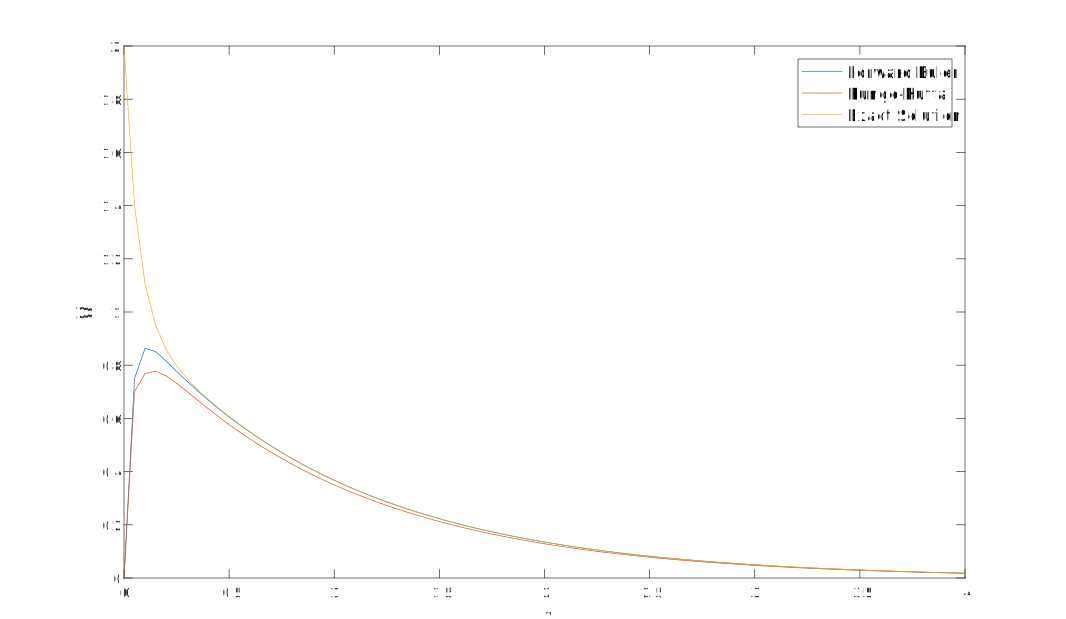
\includegraphics[width=0.99\textwidth]{Q3_both.png}
\caption{Plot of numerical solutions, Forward Euler (blue) Runge-Kutta (red), and exact solution (black)}
\label{FQ3}
\end{figure}

\section*{Question 4}
For this question I wrote Question\textunderscore4.m. It computes the data for both methods and then plots both data sets onto a single log-log graph (see Fig.\ref{FQ4}) with Euler in red and Runge-Kutta in blue. \\ \\
Theoretically the Euler method has first-order accuracy and Runge-Kutta has forth-order accuracy. Figure \ref{FQ4} supports this because the gradients of the two plots are approximately 1 and 4 for Euler and Runge-Kutta respectively.
\begin{figure}[H]
\centering
\includegraphics[width=0.99\textwidth]{Q4_both.png}
\caption{Log-log graph of $|E_n|$ against h for Forward Euler (blue) and Runge-Kutta (red)}
\label{FQ4}
\end{figure}

\section*{Question 5}
For this question I wrote Question\textunderscore5.m, below is the output. Noting that the magnitude of the global error grows exponentially the far right column shows the estimate of the growth rate after each step. \\
\begin{table}[H]
\begin{verbatim}
  x_n         Y_n            y(x_n)           E_n             gr_n 
 0.000    1.000000e+00    1.000000e+00    0.000000e+00    0.000000e+00 
 0.001    9.990000e-01    9.990005e-01   -4.998334e-07    0.000000e+00 
 0.002    9.980010e-01    9.980020e-01   -1.001166e-06    6.946463e+02 
 0.003    9.970030e-01    9.970045e-01   -1.504006e-06    4.069663e+02 
 0.004    9.960060e-01    9.960080e-01   -2.008358e-06    2.891854e+02 
   :           :               :               :               : 
 9.998   -2.155556e+13    4.549082e-05   -2.155556e+13    3.992021e+00 
 9.999   -2.164178e+13    4.544535e-05   -2.164178e+13    3.992021e+00 
10.000   -2.172835e+13    4.539993e-05   -2.172835e+13    3.992021e+00
\end{verbatim}
\caption{Output from Question\textunderscore5.m}
\end{table}

\pagebreak
Looking at this problem analytically the Euler difference equation is
\[ Y_{n+1} = Y_n + h(4Y_n - 5(e^{-h})^n) \qquad with \qquad Y_0=1 \]
This can be solved similarly to question 2 giving the solution:
\begin{align*}
Y_n &= (1+4h)^nY_0 - \frac{5h}{1-(1+4h)e^h} (e^{-nh} - (1+4h)^n) \\
Y_n &= \frac{1-5h-(1+4h)e^h}{1-(1+4h)e^h} (1+4h)^n - \frac{5h}{1-(1+4h)e^h}e^{-nh}
\end{align*}
The error comes from the $(1+4h)^n$ term, producing a growth rate of
\[ \gamma = \frac{1}{h}\ln|1+4h| \]
Therefore, for $h=0.001$ then $\gamma=\frac{1}{0.001}\ln|1+4\times0.001|\approx3.99$ which agrees with the value deduced computationally above.\\

Using a smaller value of h actually increases the growth rate fractionally rather than suppressing it. This can be understood when we thinking about the source of the error: the $(1+4h)^n$ term. Lowering h leads to a smaller (1+4h) factor but it comes at the price of increasing n which means the factor will put to a great power.
\[ As \quad h\rightarrow0 \quad then \quad \gamma\rightarrow4 \quad from\ below \]

This can be seen from plotting $\gamma = \frac{1}{h}\ln|1+4h|$.
\\ \\
Using Runge-Kutta instead of Euler would not affect the growth rate but it would lead to a smaller global error at each step. This is because RK4 is of a higher accuracy than Euler and so while the error will grow at the same rate the initial error after the first step of RK4 will be smaller than after the first step of Euler.

\section*{Question 6}

For $\alpha=4$ with $p\neq0$ the general solution is
\[ y = A(1+x)\sin(p(1+x)^{-1}-\phi) \]

if $p=0$ then
\[ y = B(1+x) \]

The particular solution (for all p) satisfying $y=0$, $dy/dx=1$ at $x=0$ is
\[ y = \frac{1}{p}(1+x)\sin(\frac{px}{1+x}) \]

Considering the alternative conditions $y(0) = y(1) = 0$
\begin{gather*}
  y(0) = 0 \quad\Rightarrow\qquad  p -\phi = m\pi \qquad m \in \mathbb{Z} \\
  y(1) = 0 \quad\Rightarrow\quad  p/2-\phi = n\pi \qquad n \in \mathbb{Z} \\
  \Rightarrow \quad p = 2\pi(m-n) = 2\pi k \qquad k \in \mathbb{Z}
\end{gather*}
Therefore the smallest (non-neg) eigenvalue with $\alpha = 4$ is $p=2\pi$. \\ \\
For eigenvalues $p=2\pi k$ with $k\in \mathbb{Z}$ then the eigenfunctions are
\[ y(x) = A_k\sin(2\pi k\frac{x}{1+x}) \]
where $A_k$ are normalization constants.

\pagebreak
\section*{Question 7}
For this question I wrote program Question\textunderscore7.m. The output for the two values of p is below.
\\ \\
Case $p=6$
\begin{table}[H]
\begin{verbatim}
                  h                 Y_n                   E_n 
               0.1/2^ 0    4.711817458469068e-02    7.8171898068e-05 
               0.1/2^ 1    4.704681924396770e-02    6.8165573453e-06 
               0.1/2^ 2    4.704046842629665e-02    4.6573967424e-07 
               0.1/2^ 3    4.704003265894316e-02    2.9972320757e-08 
               0.1/2^ 4    4.704000458071722e-02    1.8940948185e-09 
               0.1/2^ 5    4.704000280555631e-02    1.1893390439e-10 
               0.1/2^ 6    4.704000269407137e-02    7.4489650559e-12 
               0.1/2^ 7    4.704000268708800e-02    4.6559284206e-13 
               0.1/2^ 8    4.704000268665137e-02    2.8962943155e-14 
               0.1/2^ 9    4.704000268662394e-02    1.5334955528e-15 
               0.1/2^10    4.704000268662208e-02   -3.2612801348e-16 
               0.1/2^11    4.704000268662269e-02    2.8449465006e-16 
               0.1/2^12    4.704000268662233e-02   -7.6327832943e-17
\end{verbatim}
\caption{Output from Question\textunderscore7.m for $p=0.6$}
\end{table}

Case $p=7$
\begin{table}[H]
\begin{verbatim}
                  h                 Y_n                   E_n 
               0.1/2^ 0   -9.994976666384711e-02    2.7401267604e-04 
               0.1/2^ 1   -1.002052534583891e-01    1.8525881502e-05 
               0.1/2^ 2   -1.002226379990717e-01    1.1413408197e-06 
               0.1/2^ 3   -1.002237094937675e-01    6.9846123912e-08 
               0.1/2^ 4   -1.002237750360106e-01    4.3038807795e-09 
               0.1/2^ 5   -1.002237790730526e-01    2.6683877330e-10 
               0.1/2^ 6   -1.002237793232849e-01    1.6606452324e-11 
               0.1/2^ 7   -1.002237793388561e-01    1.0352829705e-12 
               0.1/2^ 8   -1.002237793398265e-01    6.4892535789e-14 
               0.1/2^ 9   -1.002237793398874e-01    3.9412917374e-15 
               0.1/2^10   -1.002237793398909e-01    4.8572257327e-16 
               0.1/2^11   -1.002237793398899e-01    1.4710455076e-15 
               0.1/2^12   -1.002237793398894e-01    1.9428902931e-15 
\end{verbatim}
\caption{Output from Question\textunderscore7.m for $p=0.7$}
\end{table}

The errors generally behave as expected. The magnitude of the global error decreases with smaller values of h. With the exception being in the $p=7$ case where the error seems to stabilise around the order of $10^{-15}$.

\pagebreak
\section*{Question 8}
For this question I wrote Question\textunderscore8.m.  Below is the equation in question.

\begin{equation}\label{EQ8}
\dv[2]{y}{x} + p^2(1+x)^{-4}y = 0
\end{equation}

Plotting a small graph (see fig.\ref{FQ8}) of exact solution at $x=1$ to equation \ref{EQ8} for p in the range $[6,7]$. We can deduce the following about the accuracy of $y_p(1)$ where $p_1$ is the first positive eigenvalue.
\begin{figure}[H]
\centering
\includegraphics[width=0.75\textwidth]{Q8.png}
\caption{Exact solution at $x=1$ to equation \ref{EQ8} for p in the range $[6,7]$}
\label{FQ8}
\end{figure}
\begin{align*}
y_p(1) &= y_{p_1}(1)+o(|p-p_1|) \\
	   &= o(|p-p_1|)
\end{align*}

Combining this with the accuracy of RK4 and that $g(p) = RK4_p(1)$ we get
\begin{align*}
|g(p)| = RK4_p(1)   &\leq \epsilon \\
y_p(1) + o(h^4) 	&\leq \epsilon \\
o(|p-p_1| + h^4) 	&\leq \epsilon
\end{align*}
Therefore in order to ensure an accuracy of at least $\pm5\times10^{-6}$ (ie $|p-p_1| \leq 5\times10^{-6}$) I took $\epsilon = 5\times10^{-6}$ and $h=1\times10^{-2}$ (s.t. $h^4=1\times10^{-8}$ which is negligible compared to $\epsilon$).

\section*{Question 9}
For this question I wrote Question\textunderscore9.m. It produces the text output below and figure \ref{FQ9a}. The programs starts at 0 and increases $x$ in steps of 5 looking for a change of sign. When it finds a sign change it uses the false-position method to find the eigenvalue within the range of that step. It then continues until it had found five eigenvalues.

\begin{verbatim}
   10.358922 
   21.263983 
   32.105846 
   42.921331 
   53.725167
\end{verbatim}

To make sure the values had the required accuracy of $\pm5\times10^{-6}$ I ran my program several times over with the RK4 step size at $h=0.01$ but each time reducing $\epsilon$, of the false-position method, by an order of magnitude until the eigenvalues being calculated stabilised to the required accuracy. This was at $\epsilon=5\times10^{-9}$.

\begin{figure}[H]
\centering
\includegraphics[width=1\textwidth]{Q9_eigenfuncs5.png}
\caption{Plot of eigenfunctions of the first five smallest eigenvalues}
\label{FQ9a}
\end{figure}

A problem could arise with the way I wrote my program if there were more than one eigenvalue in a given step of size 5. In this case only one of the eigenvalues would be found and the others ignored and so the collection of eigenvalues found by the program would not be the first five eigenvalues. To confirm that my program had not missed any eigenvalues I produced a plot of $Y_n(1)$ for p in the range $[0,100]$ (see fig.\ref{FQ9b}) from which it is possible to roughly locate the first five eigenvalues and see that none of the first five eigenvalues coincide within any one of the steps of size 5.

\begin{figure}[H]
\centering
\includegraphics[width=0.80\textwidth]{Q9_first5small.jpg}
\caption{Graph of $Y_n(1)$ calculated with $RK4$ for values of p between 0 and 100 in steps of 2}
\label{FQ9b}
\end{figure}

Studying figure \ref{FQ9a} in more detail we see several key details apart from the obvious point that all the eigenfunctions intersect at $x=0$ and $x=1$ because of the problem boundary conditions.
\\ \\
Firstly we note that in the range [0,1] all the eigenfunctions resemble sine curves with decreasing frequency and increasing amplitude. Physically they all represent normal-mode oscillations on a taught string at a fixed time. 
\begin{itemize}
\item The rate at which the frequency of each eigenfunction decreases with respect to x varies for each eigenfunction. Eigenfunctions with larger eigenvalues decrease in frequency at a slower rate. Physically this can be understood from the formula $p=\omega\ \sqrt[]{m_0/T_0}$ which shows that $\omega$, the frequency, is proportional to p.
\item The amplitude of the peaks and troughs of all the curves seem to increase in at the same rate with respect to x. This can be understood from the mass distribution function $\mu(x)=(1+x)^{-8}$ which involves string being positioned towards $x=0$ being significantly more massive than string towards $x=1$. Having a mass distribution like this significantly affects the oscillations because more massive particles have greater inertia. This means sections of string with greater mass are displaced less by the same wave compared with less massive sections of string.
\end{itemize}

% ------------------------------------------- PROGRAMS ------------------------------------------------------
\pagebreak
\section*{Programs}

\subsection*{Programming\textunderscore Task.m}
\begin{lstlisting}[style = Matlab-editor]
x = 1;                       % value to be calculated
x_0 = 0;                     % initial conditions
Y_0 = 0;           
h = 0.01;                    % size and number of steps
n = (x-x_0)/h;

fprintf("Numerical solution at x = %d with initial conditions x_0 = %d, Y_0 = %d \n",x,x_0,Y_0);
fprintf("Forward Euler: %e \n",  FE(x,n,x_0,Y_0));
fprintf("Runge-Kutta:   %e \n", RK4(x,n,x_0,Y_0));

% the function in quesiton
function[F] = f(x,y)
    F = -16*y + 15*exp(-x);
end

% Forward Euler (FE) function
function[Y] = FE(x,n,x_0,Y_0)
    h = (x-x_0)/n;
    X = x_0;
    Y = Y_0;
    for i = 1:n
        Y = Y + h*f(X,Y);
        X = X + h;
    end   
end

% Runge-Kutta (RK4) function
function[Y] = RK4(x,n,x_0,Y_0)
    h = (x-x_0)/n;
    X = x_0;
    Y = Y_0;
    for i = 0:n
        k1 = h*f(X,Y);
        k2 = h*f(X+h/2,Y+k1/2);
        k3 = h*f(X+h/2,Y+k2/2);
        k4 = h*f(X+h,Y+k3);
        Y = Y + (k1 + 2*k2 + 2*k3 + k4)/6;
        X = X + h;
    end
end
\end{lstlisting}

\pagebreak
\subsection*{Question\textunderscore1.m}
\begin{lstlisting}[style = Matlab-editor]
x = 6;                       % value to be calculated
x_0 = 0;                     % initial conditions
Y_0 = 0;
h = 0.6;                     % size and number of steps
n = (x-x_0)/h;

% Forward Euler (FE)
X = arrayfun(@(i) x_0+i*h, 0:n);
Y = [Y_0,zeros(1,n)];
for i = 2:n+1
    Y(i) = Y(i-1) + h*f(X(i-1),Y(i-1));
end
y = arrayfun(@(i) soln(x_0+i*h), 0:n); 
E = Y-y;
gr = zeros(1,n+1);
for i = 3:n+1
    gr(i) = log(abs(E(i)/E(i-1)))/h;
end

% displays data in a table
fprintf(' x_n        Y_n            y(x_n)           E_n             gr_n \n');
for i = 1:n+1
    if(i<=2)
        fprintf(' %.1f  %14.7e  %14.7e  %14.7e \n',        X(i),Y(i),y(i),E(i));
    else
        fprintf(' %.1f  %14.7e  %14.7e  %14.7e  %14.7e \n',X(i),Y(i),y(i),E(i),gr(i));
    end
end

% function in question
function[F] = f(x,y)
    F = -16*y + 15*exp(-x);
end

% exact analytic solution
function[y] = soln(x)
    y = exp(-x) - exp(-16*x);
end
\end{lstlisting}

\pagebreak
\subsection*{Question\textunderscore3.m}
\begin{lstlisting}[style = Matlab-editor]
x = 4;                       % value to be calculated
x_0 = 0;  Y_0 = 0;           % initial conditions
h = 0.05;  n = (x-x_0)/h;    % size and number of steps

% calculate data
X =          arrayfun(@(i)      x_0+i*h,            0:n);
Y_FE = [Y_0, arrayfun(@(i)   FE(x_0+i*h,i,x_0,Y_0), 1:n)];
Y_RK = [Y_0, arrayfun(@(i)  RK4(x_0+i*h,i,x_0,Y_0), 1:n)];
y =          arrayfun(@(i) soln(x_0+i*h),           0:n);

% display data in table format
fprintf(' x_n       FE Y_n         RK4 Y_n \n');
for i = 1:5
    fprintf('%2.2f    %e    %e \n',X(i),Y_FE(i),Y_RK(i));
end
fprintf('  :          :               : \n');
for i = n-1:n+1
    fprintf('%2.2f    %e    %e \n',X(i),Y_FE(i),Y_RK(i));
end

% plots the numerical solutions and exact solution
plot(X,Y_FE,    X,Y_RK,     X,y);

% function in question
function[F] = f(x,y)
    F = -16*y + 15*exp(-x);
end
% exact solution
function[y] = soln(x)
    y = exp(-x) + exp(-16*x);
end

% Forward Euler (FE) function
function[Y] = FE(x,n,x_0,Y_0)
    h = (x-x_0)/n;
    X = x_0;
    Y = Y_0;
    for i = 1:n
        Y = Y + h*f(X,Y);
        X = X + h;
    end   
end

% Runge-Kutta (RK4) function
function[Y] = RK4(x,n,x_0,Y_0)
    h = (x-x_0)/n;
    X = x_0;
    Y = Y_0;
    for i = 1:n
        k1 = h*f(X,    Y);
        k2 = h*f(X+h/2,Y+k1/2);
        k3 = h*f(X+h/2,Y+k2/2);
        k4 = h*f(X+h,  Y+k3);
        Y = Y + (k1 + 2*k2 + 2*k3 + k4)/6;
        X = X + h;
    end
end
\end{lstlisting}

\pagebreak
\subsection*{Question\textunderscore4.m}
\begin{lstlisting}[style = Matlab-editor]
x = 0.1;    % value to be calculated
x_0 = 0;    % initial conditions
Y_0 = 0;

% calculates data
h    = arrayfun(@(k) x/(2^k),0:15);
E_FE = arrayfun(@(k)  FE(x,2^k,x_0,Y_0)-soln(x),0:15);
E_RK = arrayfun(@(k) RK4(x,2^k,x_0,Y_0)-soln(x),0:15);

% displays data in table
fprintf('   h            FE E_n           RK E_n \n');
for i = 1:length(h)
    fprintf('0.1/2^%2d    %13e    %13e \n',i-1,E_FE(i),E_RK(i));
end

% plot the log-log graph of |E_n| against h
plot(log(h),log(abs(E_FE))); hold on;
plot(log(h),log(abs(E_RK)))

% function in question
function[F] = f(x,y)
    F = -16*y + 15*exp(-x);
end
% exact analytic solution
function[y] = soln(x)
    y = exp(-x) - exp(-16*x);
end

% Forward Euler (FE) function
function[Y] = FE(x,n,x_0,Y_0)
    h = (x-x_0)/n;
    X = x_0;
    Y = Y_0;
    for i = 1:n
        Y = Y + h*f(X,Y);
        X = X + h;
    end   
end

% Runge-Kutta (RK4) function
function[Y] = RK4(x,n,x_0,Y_0)
    h = (x-x_0)/n;
    X = x_0;
    Y = Y_0;
    for i = 1:n
        k1 = h*f(X,    Y);
        k2 = h*f(X+h/2,Y+k1/2);
        k3 = h*f(X+h/2,Y+k2/2);
        k4 = h*f(X+h,  Y+k3);
        Y = Y + (k1 + 2*k2 + 2*k3 + k4)/6;
        X = X + h;
    end
end
\end{lstlisting}

\pagebreak
\subsection*{Question\textunderscore5.m}
\begin{lstlisting}[style = Matlab-editor]
x   = 10;                      % value to be calculated
x_0 = 0;                       % initial conditions
Y_0 = 1;
h   = 0.001;                   % size and number of steps
n   = (x-x_0)/h;

% Forward Euler (FE) function
X = arrayfun(@(i) x_0+i*h, 0:n);
Y = [Y_0,zeros(1,n)];
for i = 2:n+1
    Y(i) = Y(i-1) + h*f(X(i-1),Y(i-1));
end
y = arrayfun(@(i) soln(x_0+i*h), 0:n); 
E = Y-y;
gr = zeros(1,n+1);
for i = 3:n+1
    gr(i) = log(abs(E(i)/E(i-1)))/h;
end

% displays data in a table
fprintf('  x_n         Y_n            y(x_n)           E_n             gr_n \n');
for i = 1:5
    fprintf('%6.3f   %13.6e   %13.6e   %13.6e   %13.6e \n',X(i),Y(i),y(i),E(i),gr(i));
end
fprintf('   :           :               :               :               : \n');
for i = n-1:n+1
    fprintf('%6.3f   %13.6e   %13.6e   %13.6e   %13.6e \n',X(i),Y(i),y(i),E(i),gr(i));
end

% function in question
function[F] = f(x,y)
    F = 4*y - 5*exp(-x);
end

% exact analytic solution
function[y] = soln(x)
    y = exp(-x);
end
\end{lstlisting}

\pagebreak
\subsection*{Question\textunderscore7.m}
\begin{lstlisting}[style = Matlab-editor]
% value to be calculated
x = 1;
% initial conditions
x_0 = 0;
Y_0 = 0;
Z_0 = 1;

% note: alpha specified as (a = 4) in function f
p = 6;

h = arrayfun(@(k) 0.1/2^k, 0:12);
Y = arrayfun(@(h) RK4(x,h,x_0,Y_0,Z_0,p), h);
E = Y - soln(x,p);

% displays data in table
fprintf('   h                 Y_n                   E_n \n');
for i = 1:length(h)
    fprintf('0.1/2^%2d   %22.15e   %17.10e \n',i-1,Y(i),E(i));
end

% function in question
function[F] = f(x,y,p)
    a = 4;
    F = [ y(2);
          -p^2*(1+x)^(-a)*y(1)];
end

% exact analytic solution
function[y] = soln(x,p)
    y = 1/p*(1+x)*sin(p*x/(1+x));
end

% Runge-Kutta (RK4) function
function[output] = RK4(x,h,x_0,Y_0,Z_0,p)
    n = (x-x_0)/h;
    X = arrayfun(@(i) x_0+i*h, 0:n);
    Y = [[Y_0;Z_0],zeros(2,n)];
    for i = 1:n
        k1 = h*f( X(i)      , Y(1:2,i)       , p);
        k2 = h*f( X(i) + h/2, Y(1:2,i) + k1/2, p);
        k3 = h*f( X(i) + h/2, Y(1:2,i) + k2/2, p);
        k4 = h*f( X(i) + h  , Y(1:2,i) + k3  , p);
        Y(1:2,i+1) = Y(1:2,i) + (k1 + 2*k2 + 2*k3 + k4)/6;
    end
    output = Y(1,n+1);
end
\end{lstlisting}

\pagebreak
\subsection*{Question\textunderscore8.m}
\begin{lstlisting}[style = Matlab-editor]
x   = 1;                  % value to be calculated
x_0 = 0;                  % initial conditions
Y_0 = 0;
Z_0 = 1;
h   = 0.01;               % size and number of steps
n   = round((x-x_0)/h);

% function for false-position method and epsilon value
g = @(p) RK4(x,h,x_0,Y_0,Z_0,p);
e = 5*10^-6;

fprintf('           p                  Y_n(1) \n');
p1 = 6;     fprintf('  %18.15f    %18.15f \n',p1, g(p1));
p2 = 7;     fprintf('  %18.15f    %18.15f \n',p2, g(p2));

p = (g(p2)*p1-g(p1)*p2)/(g(p2)-g(p1));
while(abs(g(p)) > e)
    if(sign(g(p)*g(p1)) == 1)
        p1 = p;
    else
        p2 = p;
    end
    p = (g(p2)*p1-g(p1)*p2)/(g(p2)-g(p1));
    fprintf('  %18.15f    %18.15f \n',p, g(p));
end

% the plot for the figure included in question 8
fplot(@(p) soln(1,p),[6,7]);

% function in question
function[F] = f(x,y,p)
    a = 4;
    F = [ y(2);
          -p^2*(1+x)^(-a)*y(1)];
end

% exact analytic solution
function[y] = soln(x,p)
    y = 1/p*(1+x)*sin(p*x/(1+x));
end

% Runge-Kutta (RK4) function
function[output] = RK4(x,h,x_0,Y_0,Z_0,p)
    n = round((x-x_0)/h);
    X = arrayfun(@(i) x_0+i*h, 0:n);
    Y = [[Y_0;Z_0],zeros(2,n)];
    for i = 1:n
        k1 = h*f( X(i)      , Y(1:2,i)       , p);
        k2 = h*f( X(i) + h/2, Y(1:2,i) + k1/2, p);
        k3 = h*f( X(i) + h/2, Y(1:2,i) + k2/2, p);
        k4 = h*f( X(i) + h  , Y(1:2,i) + k3  , p);
        Y(1:2,i+1) = Y(1:2,i) + (k1 + 2*k2 + 2*k3 + k4)/6;
    end
    output = Y(1,n+1);
end
\end{lstlisting}

\pagebreak
\subsection*{Question\textunderscore9.m}
\begin{lstlisting}[style = Matlab-editor]
x = 1;                  % value to be calculated
x_0 = 0;                % initial conditions
Y_0 = 0;
Z_0 = 1;
h = 0.01;               % number and size of steps
n = (x-x_0)/h;
a = 8;                  % alpha
N = 5;                  % number of eigen-values to find
P = zeros(1,N);         % eigenvalues
C = zeros(1,N);         % scaling constants for eigenfunctions

% function for false position method
g = @(p) RK4(x,h,x_0,Y_0,Z_0,a,p);

s  = 5;                 % step size
p1 = 0;                 % starting step
p2 = p1 + s;
for i=1:N
    while(g(p1)*g(p2)>0)
        p2 = p2 + s;
        p1 = p1 + s;
    end
    P(i) = FP(x,h,x_0,Y_0,Z_0,a,p1,p2);
    fprintf('%f \n',P(i));
    p2 = p2 + s;
    p1 = p1 + s;
    X = (0:0.01:1);
    I = @(x) (1+x)^-8*RK4(x,h,x_0,Y_0,Z_0,a,P(i))^2;
    C(i) = (p^2*trapz(X,arrayfun(I,X)))^(-1/2);
end

% plot of the first five smallest eigenfunctions
y = @(p) @(x) RK4(x,0.01,x_0,Y_0,Z_0,a,p);
x = (0:0.01:1);
plot(x,C(1)*arrayfun(y(P(1)),x)); hold on;
plot(x,C(2)*arrayfun(y(P(2)),x)); hold on;
plot(x,C(3)*arrayfun(y(P(3)),x)); hold on;
plot(x,C(4)*arrayfun(y(P(4)),x)); hold on;
plot(x,C(5)*arrayfun(y(P(5)),x)); hold on;

% uncomment the code below for plot to verify where the first five smallest eigenvalues lie
% x = (0:2:100);
% plot(x,arrayfun(g,x));

% false position function
function[p] =  FP(x,h,x_0,Y_0,Z_0,a,p1,p2)
    g = @(p) RK4(x,h,x_0,Y_0,Z_0,a,p);
    e = 5*10^-9;
    p = (g(p2)*p1-g(p1)*p2)/(g(p2)-g(p1));
    while(abs(g(p)) > e)
        p = (g(p2)*p1-g(p1)*p2)/(g(p2)-g(p1));
        if(sign(g(p)*g(p1)) == 1)
            p1 = p;
        else
            p2 = p;
        end
    end
end

% function in question
function[F] = f(x,y,a,p)
    F = [ y(2);
          -p^2*(1+x)^(-a)*y(1)];
end

% Runge-Kutta (RK4) function
function[output] = RK4(x,h,x_0,Y_0,Z_0,a,p)
    n = round((x-x_0)/h);
    if(n>0)
        X = arrayfun(@(i) x_0+i*h, 0:n);
        Y = [[Y_0;Z_0],zeros(2,n)];
        for i = 1:n
            k1 = h*f( X(i)      , Y(1:2,i)       , a, p);
            k2 = h*f( X(i) + h/2, Y(1:2,i) + k1/2, a, p);
            k3 = h*f( X(i) + h/2, Y(1:2,i) + k2/2, a, p);
            k4 = h*f( X(i) + h  , Y(1:2,i) + k3  , a, p);
            Y(1:2,i+1) = Y(1:2,i) + (k1 + 2*k2 + 2*k3 + k4)/6;
        end
        output = Y(1,n+1);
    else
        output = Y_0;
    end
end
\end{lstlisting}

\end{document}














